\documentclass[
  headings=standardclasses,
  bibliography=totocnumbered,
]{scrartcl}

\usepackage{../../common/common_packages}
\usepackage{../../common/macros}
\usepackage{../../common/theorem_styles}
\usepackage{../../common/colors}

% Misc packages
\usepackage{tikz}
\usepackage{float} % Allow figures inside minipages

% Bibliography
\addbibresource{./references.bib}

% Setup TikZ
\usetikzlibrary{arrows.meta}

% Document
\title{\Title{1}}
\subtitle{Уравнение на права и равнина. Формули за разстояния и ъгли. Криви от втора степен.}
\author{Янис Василев}
\date{\Revision{11 юни 2019}}

\begin{document}

\maketitle

\section{Теория}

Теорията е до голяма степен базирана на \cite{Notes}.

\subsection{Анотация}

Изложената анотацията е взета от \cite{Syllabus}.

\begin{enumerate}
  \item Прави в равнината и пространството
  \begin{enumerate}
    \item Векторни и параметрични (скаларни) уравнения на права и равнина
    \item Общо уравнение на права в равнината
    \item Декартово уравнение
    \item Взаимно положение на две прави
    \item Нормално уравнение на права
    \item Разстояние от точка до права
    \item Ъгъл между прави
  \end{enumerate}

  \item Равнини в пространството
  \begin{enumerate}
    \item Общо уравнение на равнина
    \item Взаимно положение на две равнини
    \item Нормално уравнение на равнина
    \item Разстояние от точка до равнина
  \end{enumerate}

  \item Криви от втора степен
  \begin{enumerate}
    \item Уравнение на окръжност
    \item Канонични уравнения на елипса, хипербола и парабола
    \item Фокални свойства на елипса, хипербола и парабола
  \end{enumerate}
\end{enumerate}

\subsection{Прави в равнината}

Нека \( K = Oxy \) е афинна координатна система в равнината \( A_2 \). Считаме, че е зададена единична отсечка за измерване на дължини.

\begin{definition}
  Нека \( l \) е права в \( A_2 \), нека са дадени \( \Point P_0 \in l \) и направляващият за \( l \) вектор \( v \parallel l \). Очевидно векторът \( v \) е ненулев. Нека \( r_0 = \V{OP_0} \) и \( r = \V{OP} \) са радиус-векторите на точките \( \Point P_0 \) и \( \Point P \) спрямо \( K \).

  От тъждествата \( r - r_0 = \V{P_0 P} \parallel v \iff P \in l \) и \( \forall \lambda \in \R : v \parallel \lambda v \) следва, че правата \( l \) удовлетворява уравнението
  \begin{equation*}
    l: r = r_0 + \lambda v, \lambda \in \R,
  \end{equation*}
  което наричаме \textbf{векторно параметрично уравнение} на \( l \) спрямо \( K \).

  Нека \( \Point P_0 \), \( \Point P \) и \( v \) имат координати \( P_0(x_0, y_0) \), \( P(x, y) \) и \( v(a, b) \) спрямо \( K \). Уравненията
  \begin{equation*}
    l: \begin{cases}
      x = x_0 + \lambda a \\
      y = y_0 + \lambda b
    \end{cases},
    \lambda \in \R
  \end{equation*}
  наричаме \textbf{система скаларни параметрични уравнения} на \( l \) спрямо \( K \).
\end{definition}

Изхождайки от горната система, имаме \( \lambda a b = b(x - x_0) = a(y - y_0) \), откъдето получаваме уравнението \( l: bx + (-a)y + (-x_0 + y_0) = 0 \).

\begin{definition}
  Нека правата \( l \) се задава спрямо \( K \) с уравнението \( l: Ax + By + C = 0 \), където \( A, B, C \in \R \), т.е. уравнението е изпълнено за координатите на \( \Point P(x, y) \) точно когато \( \Point P \in l \).

  Уравнение от този вид наричаме \textbf{общо уравнение на правата} \( l \) спрямо \( K \).
\end{definition}

\begin{remark}
  От определението е ясно, че е изпълнено \( A \neq 0 \) или \( B \neq 0 \), тъй като в противен случай уравнението е еквивалентно на \( l: C = 0 \) и, в зависимост от стойността на \( C \), уравнението задава или празното множество, или цялата равнина \( A_2 \).
\end{remark}

Вече видяхме, че от всяка система скаларни параметрични уравнение за права \( l \) можем да намерим поне едно общо уравнение за \( l \). Ще докажем съществуване на общо уравнение за равнина по друг начин.

\begin{proposition}
  Всяко уравнение от вида \( Ax + By + C = 0 \), където \( A \) и \( B \) не са едновременно равни на \( 0 \), е уравнение на точно една права спрямо \( K \).
\end{proposition}
\begin{proof}
  Без ограничение на общността допускаме, че \( A \neq 0 \).

  Да забележим, че уравнението има поне едно решение, например \( x = -\frac C A \) и \( y = 0 \).

  Нека е дадена точката \( P_0(x_0, y_0) \), чиито координати удовлетворяват уравнението. Нека \( v \) е ненулевият вектор с координати \( v(B, -A) \). Тогава системата
  \begin{equation*}
    l: \begin{cases}
      x = x_0 + \lambda B \\
      y = y_0 - \lambda A,
    \end{cases}
    \lambda \in \R
  \end{equation*}
  е система скаларни параметрични уравнения за някаква права \( l \). Ще покажем, че тази система е еквивалентна на даденото уравнение.

  От една страна, всяко решение на общото уравнение удовлетворява системата, тъй като \( C = -Ax_0 - By_0 \). Получаваме
  \begin{align*}
    Ax + By + C &= 0, \\
    x &= -\frac C A -\frac {By} A, \\
    x &= \frac {Ax_0 + By_0} A -\frac {By} A, \\
    x &= x_0 + \frac {y_0 - y} A B.
  \end{align*}

  Полагаме \( \lambda \coloneqq \frac{y_0 - y} A \), откъдето получаваме
  \begin{equation*}
    \begin{cases}
      x = x_0 + \lambda B \\
      y = y_0 - \lambda A
    \end{cases}.
  \end{equation*}

  От друга страна, всяко решение на системата удовлетворява общото уравнение, тъй като
  \begin{equation*}
    A (x_0 + \lambda B) + B (y_0 - \lambda A) + C
    =
    (A x_0 + B y_0 + C) + (\lambda AB - \lambda AB)
    =
    0 + 0 = 0.
  \end{equation*}
\end{proof}

\begin{definition}
  Нека правата \( l \) има спрямо \( K \) общо уравнение \( l: Ax + By + C = 0 \). Нека още \( l \) не е успоредна на оста \( Oy \). Тогава \( B \neq 0 \) и можем да запишем общото уравнение във вида

  \begin{align*}
    l: \frac A B x + y + \frac C B = 0
    &&\sim&&
    l: y = \left(-\frac A B \right) x + \left(-\frac C B \right).
  \end{align*}

  Полагаме \( k = -\frac A B \) и \( m = -\frac C B \). Уравнението
  \begin{equation*}
    l: y = kx + m
  \end{equation*}
  наричаме \textbf{декартово уравнение} на \( l \) спрямо \( K \), а коефициента \( k \) наричаме \textbf{ъглов коефициент} на \( l \) спрямо \( K \).
\end{definition}

\begin{definition}
  \mbox{}
  \begin{enumerate}
    \item \textbf{Ъгъл между две пресекателни прави} наричаме по-малкия от двата ъгъла, които те сключват.

    Ако е зададена ориентация, \textbf{ориентиран ъгъл между пресекателни прави} наричаме ъгъла, на който трябва да бъде завъртяна спрямо зададената ориентация първата права около пресечната си точка с втората права, за да съвпадне с нея.

    \item \textbf{Ъгъл между два лъча с общо начало} наричаме по-малкия от двата ъгъла, които те сключват.

    \textbf{Ориентиран ъгъл между два лъча с общо начало} наричаме ъгъла, на който трябва да бъде завъртян спрямо зададената ориентация първият лъч относно началната си точка, за да съвпадне с втория.

    \item Нека са дадени ненулеви свободните вектори \( u \) и \( v \). \textbf{Ъгъл между \( u \) и \( v \)} наричаме по-малкия от двата ъгъла между два произволни техни представителя с общо начало и бележим с \( \angle(u, v) \).

    \textbf{Ориентиран ъгъл между \( u \) и \( v \)} наричаме ъгъла, на който трябва да бъде завъртян някой представител на \( u \) спрямо зададената ориентация, за да съвпадне с някой представител на \( v \).

    И двете дефиниции са коректни, понеже всички представители на \( u \) са колинеарни помежду си и сключват еднакви ъгли с представители на \( v \), които също са колинеарни помежду си.
  \end{enumerate}
\end{definition}

\begin{proposition}
  Нека координатната система \( K = Oxy \) е ортонормирана и правата \( l \) има спрямо \( K \) декартово уравнение \( l: y = kx + m \). Дефинираме лъчът \( r\Ray : y = kx + m \geq 0 \), лежащ върху \( l \). Тогава \( \tan \angle(r\Ray, Ox\Ray) = k \).
\end{proposition}
\begin{proof}
  Нека \( u \) е векторът с координати \( u(1, k) \) спрямо \( K \).

  Ако \( k \geq 0 \), то \( u \upuparrows r\Ray \) и
  \begin{equation*}
     \tan \angle(r\Ray, Ox\Ray) = \tan \angle(u, Ox\Ray) = k.
  \end{equation*}

  Ако \( k < 0 \), то \( u \updownarrows r\Ray \) и
  \begin{equation*}
    \tan \angle(r\Ray, Ox\Ray) = \tan(\pi - \angle(-u, Ox\Ray)) = -\tan \angle(-u, Ox\Ray) = -(-k) = k.
  \end{equation*}
\end{proof}

\begin{theorem}
  Нека правите \( l_1 \) и \( l_2 \) имат спрямо \( K \) общи уравнения
  \begin{equation}\label{thm:plane_line_position/scalar_equations}
    l_i : A_i x + B_i y + C_i, i = 1, 2.
  \end{equation}

  Означаваме

  \begin{align*}
    L \coloneqq \begin{pmatrix}
      A_1 & B_1 \\
      A_2 & B_2
    \end{pmatrix}
    &&
    \tilde L \coloneqq \begin{pmatrix}
      A_1 & B_1 & C_1 \\
      A_2 & B_2 & C_2
    \end{pmatrix}.
  \end{align*}

  Тогава
  \begin{enumerate}
    \item \( l_1 \equiv l_2 \iff \Rank L = \Rank \tilde L = 1 \).
    \item \( l_1 \parallel l_2 \), но \( l_1 \not\equiv l_2 \iff 1 = \Rank L < \Rank \tilde L = 2 \).
    \item \( l_1 \) и \( l_2 \) са пресекателни \( \iff \Rank L = \Rank \tilde L = 2 \).
  \end{enumerate}
\end{theorem}
\begin{proof}
  Да забележим, че
  \begin{enumerate}
    \item \( L \) е подматрица на \( \tilde L \implies \Rank L \leq \Rank \tilde L \).
    \item \( A_1 \) и \( B_1 \) са коефициенти в общо уравнения на права, съответно поне един от тях е различен от нула и \( \Rank L \geq 1 \).
    \item Матрицата \( \tilde L \) има само два реда, следователно \( \Rank \tilde L \leq 2 \).
  \end{enumerate}

  Така получаваме \( 1 \leq \Rank L \leq \Rank \tilde L \leq 2 \).

  Разглеждаме матричното уравнение
  \begin{equation}\label{thm:plane_line_position/matrix_equation}
    L
    \begin{pmatrix}
      x \\ y \\ 1
    \end{pmatrix}
    =
    \begin{pmatrix}
      -C_1 \\ -C_2
    \end{pmatrix},
  \end{equation}
  което ни дава едновременните решения на уравненията (\eqref{thm:plane_line_position/scalar_equations}).

  Ако \( \Rank L \neq \Rank \tilde L \), то по теоремата на Руше матричното уравнение (\eqref{thm:plane_line_position/matrix_equation}) няма решение, правите \( l_1 \) и \( l_2 \) нямат общи точки и \( l_1 \parallel l_2 \). Обратно, ако правите са успоредни, те нямат общи точки, матричното уравнение (\eqref{thm:plane_line_position/matrix_equation}) няма решения и \( \Rank L \neq \Rank \tilde L \).

  Ако \( \Rank L = \Rank \tilde L \), то по теоремата на Руше матричното уравнение (\eqref{thm:plane_line_position/matrix_equation}) има поне едно решение. Разглеждаме два случая:
  \begin{enumerate}
    \item Ако \( \Rank L = \Rank \tilde L = 1 \), то редовете на \( L \) са линейно зависими, следователно уравненията (\eqref{thm:plane_line_position/scalar_equations}) са еквивалентни и задават едно и също множество. Тъй като и двете са уравнения на прави, те задават една и съща права.

    Обратно, нека уравненията (\eqref{thm:plane_line_position/scalar_equations}) задават една и съща права и нека за определеност \( A_1 \neq 0 \). Тогава за произволна точка \( P(x, y) \in l_1 \equiv l_2 \) имаме
    \begin{equation*}
      A_1x + B_1y + C_1 = 0
      \implies
      x = - \frac {B_1} {A_1} y - \frac {C_1} {A_1},
    \end{equation*}
    \begin{align*}
      A_2x + B_2y + C_2 &= 0,
      \\
      - A_2 \left(\frac {B_1} {A_1} y + \frac {C_1} {A_1} \right) + B_2y + C_2 &= 0,
      \\
      \left(B_2 - \frac {A_2} {A_1} B_1 \right) y + \left(C_2 - \frac {A_2} {A_1} C_1 \right) &= 0.
    \end{align*}

    Последното уравнение е еквивалентно на системата
    \begin{align*}
      B_2 = \frac {A_2} {A_1} B_1
      &&
      C_2 = \frac {A_2} {A_1} C_1.
    \end{align*}

    Тогава второто уравнение от (\eqref{thm:plane_line_position/scalar_equations}) има вида
    \begin{equation*}
      l_2:
      A_2 x + B_2 y + C_2 =
      \frac {A_2} {A_1} A_1 x + \frac {A_2} {A_1} B_1 y + \frac {A_2} {A_1} C_1
      = 0,
    \end{equation*}
    откъдето виждаме, че двете уравнения са пропорционални и следователно \( \Rank \tilde L = 1 \).

    \item Ако \( \Rank L = \Rank \tilde L = 2 \), то системата (\eqref{thm:plane_line_position/matrix_equation}) има максимален ранг и решението е единствено. Това е пресечната точка на \( l_1 \) и \( l_2 \).

    Обратно, ако \( l_1 \) и \( l_2 \) имат само една обща точка \( P \), то координатите ѝ удовлетворяват (\eqref{thm:plane_line_position/matrix_equation}). По теоремата на Руше това или е единственото решение, или има още безброй решения. Но вече видяхме, че системата има безброй решения точно при \( \Rank \tilde L = 1 \). Следователно координатите на \( P \) са единственото решение на (\eqref{thm:plane_line_position/matrix_equation}) и матрицата \( L \) има максимален ранг 2.
  \end{enumerate}
\end{proof}

\begin{corollary}
  Ако правата \( l \) има общо уравнение \( l: Ax + By + C = 0 \) спрямо \( K \), то всяко общо уравнение спрямо \( K \) има вида \( l: \lambda(Ax + By + C) = 0 \) за някое \( \lambda \in \R \setminus \{ 0 \} \).
\end{corollary}

\begin{definition}
  Всеки вектор, перпендикулярен на някоя права \( l \), се нарича \textbf{нормален} за \( l \).
\end{definition}

\begin{proposition}
  Ако правата \( l \) има общо уравнение \( l: Ax + By + C = 0 \) спрямо \( K \) и \( K \) е ортонормирана, то
  \begin{enumerate}
    \item векторът \( v(-B, A) \) е ненулев и колинеарен с \( l \).
    \item векторът \( n(A, B) \) е ненулев и нормален за \( l \).
  \end{enumerate}
\end{proposition}
\begin{proof}
  По условие имаме, че \( A \) и \( B \) не са едновременно равни на \( 0 \), следователно \( v \) и \( n \) са ненулеви.
  \begin{enumerate}
    \item Разглеждаме точката \( P_0(x_0, y_0) \in l \) и точката \( P_1(x_0 - B, y_0 + A) \), която също принадлежи на \( l \), тъй като
    \begin{equation*}
      A(x_0 - B) + B(y_0 + A) + C = (Ax_0 + By_0 + C) + (-AB + AB) = 0 + 0 = 0.
    \end{equation*}
     Тогава \( \V{P_0 P_1} \parallel l \). Но векторът \( \V{P_0 P_1}(-B, A) \) е равен на \( v \), следователно \( v \parallel l \).

    \item Тъй като координатната система \( K \) е ортонормирана, имаме
    \begin{equation*}
      \Prod v n = -AB + AB = 0,
    \end{equation*}
    следователно \( v \perp n \) и тъй като \( v \) е направляващ за \( l \), то \( n \) е нормален за \( l \).
  \end{enumerate}
\end{proof}

\begin{definition}
  Общото уравнение \( l: \alpha x + \beta y + \gamma = 0 \) на права \( l \) спрямо ортонормирана \( K \) се нарича \textbf{нормално}, ако е изпълнено условието \( \Norm{n(\alpha, \beta)}^2 = \alpha^2 + \beta^2 = 1 \).
\end{definition}

\begin{proposition}
  Всяка права има спрямо \( K \) точно две нормални уравнения.
\end{proposition}
\begin{proof}
  Нека \( l \) има спрямо \( K \) общо уравнение \( l: Ax + By + C = 0 \). Тогава всевъзможните общи уравнения на \( l \) спрямо \( K \) имат вида
  \begin{equation*}
    l: \lambda(Ax + By + C) = 0, \lambda \in \R \setminus \{ 0 \}.
  \end{equation*}

  Но \( {(\lambda A)}^2 + {(\lambda B)}^2 = 1 \iff \lambda = \pm \frac 1 {\sqrt{A^2 + B^2}} \).

  Двете нормални уравнения са
  \begin{equation*}
    l: \pm \frac {Ax + By + C} {\sqrt{A^2 + B^2}} = 0.
  \end{equation*}
\end{proof}

\begin{theorem}\label{thm:plane_distance}
  Нека координатната система \( K \) е ортонормирана и са дадени точката \( P_0(x_0, y_0) \) и правата \( l \) с нормално уравнение
  \begin{equation*}
    l: \alpha x + \beta y + \gamma = 0.
  \end{equation*}

  Означаваме \( F(x, y) \coloneqq \alpha x + \beta y + \gamma \). Тогава разстоянието между \( P_0 \) и \( l \) е
  \begin{equation*}
    \Dist(P_0, l) = \Abs{F(x_0, y_0)},
  \end{equation*}
  а величината \( \ODist(P, l) = F(x_0, y_0) \) се нарича \textbf{ориентирано разстояние} между \( P_0 \) и \( l \).
\end{theorem}
\begin{proof}
  Нека \( P_1(x_1, y_1) \) е ортогоналната проекция на \( P_0 \) върху \( l \). Понеже \( \V{P_0 P_1} \perp l \), то \( \V{P_0 P_1} \parallel n(\alpha, \beta) \), следователно \( \exists \lambda \in \R: \V{P_0 P_1} = \lambda n \). Тогава
  \begin{equation*}
    \Dist(P_0, l)
    =
    \Norm{\V{P_0 P_1}}
    =
    \Abs{\lambda} \Norm{n}
    =
    \Abs{\lambda}.
  \end{equation*}

  Намираме \( \lambda \) от \( \V{P_0 P_1}(x_1 - x_0, y_1 - y_0) = \lambda n(\alpha, \beta) \):
  \begin{equation*}
    \begin{cases}
      x_1 - x_0 = \lambda \alpha \\
      y_1 - y_0 = \lambda \beta
    \end{cases}
    \sim
    \begin{cases}
      x_1 = x_0 + \lambda \alpha \\
      y_1 = y_0 + \lambda \beta.
    \end{cases}
  \end{equation*}

  Заместваме в нормалното уравнение на \( l \):
  \begin{align*}
    \alpha x_1 + \beta y_1 + \gamma &= 0,
    \\
    \alpha (x_0 + \lambda \alpha) + \beta (y_0 + \lambda \beta) + \gamma &= 0,
    \\
    (\alpha x_0 + \beta y_0 + \gamma) + \lambda(\alpha^2 + \beta^2) &= 0,
    \\
    F(x_0, y_0) + \lambda &= 0,
  \end{align*}
  откъдето следва \( \lambda = -F(x_0, y_0) \) и \( \Dist(P_0, l) = \Abs{\lambda} = \Abs{F(x_0, y_0)} \).
\end{proof}

\begin{theorem}
  Нека са дадени правите \( l_1 \) и \( l_2 \) с нормални уравнения спрямо ортонормирана \( K \)
  \begin{equation*}
    l_i: \alpha_i x + \beta_i y + \gamma_i = 0, i = 1, 2.
  \end{equation*}

  Тогава за ъгълът между \( l_1 \) и \( l_2 \) е \( \angle(l_1, l_2) = \arccos \Abs{\alpha_1 \alpha_2 + \beta_1 \beta_2} \).
\end{theorem}
\begin{proof}
  Нека векторите \( n_i(\alpha_i, \beta_i) \) са нормални за \( n_i, i = 1, 2 \).

  Разглеждаме два случая:
  \begin{enumerate}
    \item Ако \( 0 < \angle(n_1, n_2) \leq \frac {\pi} 2 \), то \( \angle(l_1, l_2) = \angle(n_1, n_2) \) и
    \begin{equation*}
      \cos \angle (l_1, l_2)
      =
      \cos \angle(n_1, n_2)
      =
      \Abs{\cos \angle (n_1, n_2)}.
    \end{equation*}

    \item Ако \( \frac {\pi} 2 < \angle(n_1, n_2) \leq \pi \), то \( \angle(l_1, l_2) = \pi - \angle(n_1, n_2) \)
    \begin{equation*}
      \cos \angle (l_1, l_2)
      =
      \cos (\pi - \angle(n_1, n_2))
      =
      -\cos \angle(n_1, n_2)
      =
      \Abs{\cos \angle (n_1, n_2)}.
    \end{equation*}
  \end{enumerate}

  И в двата случая имаме
  \begin{equation*}
    \cos \angle(l_1, l_2)
    =
    \Abs{\cos \angle(n_1, n_2)}
    =
    \frac {\Abs {\Prod {n_1} {n_2}}} {\Norm{n_1} \Norm{n_2}}
    =
    \Abs{\alpha_1 \alpha_2 + \beta_1 \beta_2}
  \end{equation*}
  и
  \begin{equation*}
    \angle(l_1, l_2)
    =
    \arccos \Abs{\alpha_1 \alpha_2 + \beta_1 \beta_2}.
  \end{equation*}
\end{proof}

\subsection{Равнини в пространството}

\begin{remark}
  Някои от теоремите са напълно аналогични на тези за прави в равнината и ще пропуснем техните доказателства.
\end{remark}

Нека \( K = Oxyz \) е афинна координатна система в пространството \( A_3 \). Считаме, че е зададена единична отсечка за измерване на дължини.

\begin{definition}
  Нека равнината \( \pi \) се задава спрямо \( K \) с уравнението \( \pi: Ax + By + Cz + D = 0 \), където \( A, B, C, D \in \R \), т.е. уравнението е изпълнено за координатите на \( \Point P(x, y, z) \) точно когато \( \Point P \in \pi \).

  Уравнение от този вид наричаме \textbf{общо уравнение на равнината \( \pi \)} спрямо \( K \).
\end{definition}

\begin{remark}
  От определението е ясно, че е изпълнено \( A \neq 0 \) или \( B \neq 0 \) или \( C \neq 0 \), тъй като в противен случай уравнението е еквивалентно на \( l: D = 0 \) и, в зависимост от стойността на \( D \), уравнението задава или празното множество, или цялото пространство \( A_3 \).
\end{remark}

\begin{proposition}
  \mbox{}
  \begin{enumerate}
    \item Всяка равнина има поне едно общо уравнение спрямо \( K \).
    \item Всяко уравнение от вида \( Ax + By + Cz + D = 0 \), където \( A \), \( B \) и \( C \) не са едновременно равни на \( 0 \), е уравнение точно една равнина спрямо \( K \).
  \end{enumerate}
\end{proposition}
\begin{proof}
  \mbox{}
  \begin{enumerate}
    \item Нека са дадени равнината \( \pi \), точката \( P_0(x_0, y_0, z_0) \in \pi \) и компланарните с \( \pi \) неколинеарни вектори \( u_i(a_i, b_i, c_i), i = 1, 2 \).

    Разглеждаме произволна точка \( P(x, y, z) \). Имаме \( \Point P \in l \) точно когато \( \V{P_0 P} \parallel \pi \), а последното условие е аналогично на това векторите \( \V{P_0 P} \), \( u_1 \) и \( u_2 \) да бъдат компланарни. Това условие може да се изрази в координатен вид,
    \begin{align*}
      \det \begin{pmatrix}
        x - x_0 & a_1 & a_2 \\
        y - y_0 & b_1 & b_2 \\
        z - z_0 & c_1 & c_2 \\
      \end{pmatrix}
      =
      0.
    \end{align*}
    Полагаме
    \begin{align*}
      A \coloneqq \det \begin{pmatrix}
        b_1 & b_2 \\
        c_1 & c_2
      \end{pmatrix}
      &&
      B \coloneqq -\det \begin{pmatrix}
        a_1 & a_2 \\
        c_1 & c_2
      \end{pmatrix}
      &&
      C \coloneqq \det \begin{pmatrix}
        a_1 & a_2 \\
        b_1 & b_2
      \end{pmatrix}.
    \end{align*}
    Тъй като векторите \( u_1 \) и \( u_2 \) не са колинеарни, имаме
    \begin{align*}
      \Rank \begin{pmatrix}
        a_1 & a_2 \\
        b_1 & b_2 \\
        c_1 & c_2 \\
      \end{pmatrix} = 2,
    \end{align*}
    следователно поне едно от адюнгираните количества \( A \), \( B \) или \( C \) на голямата матрица ще бъде различно от \( 0 \).

    След като разложим пресмятането на детерминантата по първия стълб, можем да запишем полученото уравнение във вида
    \begin{align*}
      \det \begin{pmatrix}
        x - x_0 & a_1 & a_2 \\
        y - y_0 & b_1 & b_2 \\
        z - z_0 & c_1 & c_2 \\
      \end{pmatrix}
      =
      Ax + By + Cz - (Ax_0 + By_0 + Cz_0) = 0,
    \end{align*}
    откъдето след полагането \( D \coloneqq - (Ax_0 + By_0 + Cz_0) \) получаваме общо уравнение за \( \pi \).

    \item Нека е дадено уравнението \( Ax + By + Cz + D = 0 \), където \( A \), \( B \) и \( C \) не са едновременно равни на \( 0 \). Без ограничение на общността допускаме, че \( A \neq 0 \).

    Да забележим, че уравнението има поне едно решение, например \( x = -\frac D A \) и \( y = z = 0 \).

    Нека са дадени векторите \( u_1(-B, A, 0) \) и \( u_2 \left(-\frac C A, 0, 1 \right) \) и точките \( P_0(x_0, y_0, z_0) \) и \( P(x, y, z) \). Нека освен това координатите на \( P_0 \) удовлетворяват уравнението. Тогава \( D = -(Ax_0 + By_0 + Cz_0) \).

    Нека \( \pi \) е равнината, образувана от векторите \( u_1 \) и \( u_2 \). Тогава \( \V{P_0 P} \in \pi \iff \) трите вектора са компланарни. Ако изразим това условие в координатен вид, ще получим оригиналното уравнение. Наистина,
    \begin{align*}
      &\det \begin{pmatrix}
        x - x_0 & -B & -\frac C A \\
        y - y_0 & A & 0 \\
        z - z_0 & 0 & 1 \\
      \end{pmatrix}
      = \\ &=
      Ax + By + Cz - (Ax_0 + By_0 + Cz_0)
      = \\ &=
      Ax + By + Cz + D = 0.
    \end{align*}

    Следователно \( Ax + By + Cz + D \) е уравнение на равнината \( \pi \) спрямо \( K \).
  \end{enumerate}
\end{proof}

\begin{theorem}
  Нека правите \( \alpha_1 \) и \( \alpha_2 \) имат спрямо \( K \) общи уравнения
  \begin{equation}
    \pi_i : A_i x + B_i y + C_i z + D_i, i = 1, 2.
  \end{equation}

  Означаваме

  \begin{align*}
    L \coloneqq \begin{pmatrix}
      A_1 & B_1 & C_1 \\
      A_2 & B_2 & C_2
    \end{pmatrix}
    &&
    \tilde L \coloneqq \begin{pmatrix}
      A_1 & B_1 & C_1 & D_1 \\
      A_2 & B_2 & C_2 & D_2
    \end{pmatrix}.
  \end{align*}

  Тогава
  \begin{enumerate}
    \item \( \pi_1 \equiv \pi_2 \iff \Rank L = \Rank \tilde L = 1 \).
    \item \( \pi_1 \parallel \pi_2 \), но \( \pi_1 \not\equiv \pi_2 \iff 1 = \Rank L < \Rank \tilde L = 2 \).
    \item \( \pi_1 \) и \( \pi_2 \) са пресекателни \( \iff \Rank L = \Rank \tilde L = 2 \).
  \end{enumerate}
\end{theorem}

\begin{definition}
  Всеки вектор, перпендикулярен на някоя равнина \( \pi \), се нарича \textbf{нормален} за \( \pi \).
\end{definition}

\begin{proposition}
  Ако равнината \( \pi \) има общо уравнение \( \pi: Ax + By + Cz + D = 0 \) спрямо \( K \) и \( K \) е ортонормирана, то
  \begin{enumerate}
    \item векторите \( u(-B, A, 0) \) и \( v(-C, 0, A) \) са неколинеарни, ненулеви и компланарни с \( \pi \).
    \item векторът \( n(A, B, C) \) е ненулев и нормален за \( l \).
  \end{enumerate}
\end{proposition}
\begin{proof}
  \item Разглеждаме точката \( P_0(x_0, y_0, z_0) \in l \) и точките
  \begin{align*}
    P_1(x_0 - B, y_0 + A, z_0)
    &&
    P_2(x_0 - C, y_0, z_0 + A),
  \end{align*}
  които също принадлежат на \( l \), тъй като
  \begin{align*}
    &A(x_0 - B) + B(y_0 + A) + Cz_0 + D = (Ax_0 + By_0 + Cz_0 + D) + (-AB + AB) = 0, \\
    &A(x_0 - C) + By_0 + C(z_0 + A) + D = (Ax_0 + By_0 + Cz_0 + D) + (-AC + AC) = 0.
  \end{align*}

  Тогава векторите \( \V{P_0 P_1} \) и \( \V{P_0 P_2} \) са компланарни с \( \pi \). Но \( \V{P_0 P_1} = u \) и \( \V{P_0 P_2} = v \), следователно \( u \) и \( v \) са компланарни с \( \pi \).

  \item Тъй като координатната система \( K \) е ортонормирана, имаме
  \begin{equation*}
    \Prod u n = -AB + AB = 0 = -AC + AC = \Prod v n,
  \end{equation*}
  следователно \( u \perp n \) и \( v \perp n \). Тогава \( n \) е перпендикулярен и на всички линейни комбинации на \( u \) и \( v \) и понеже \( u \) и \( v \) образуват равнината \( \pi \), то \( n \) е нормален за \( \pi \).
\end{proof}

\begin{definition}
  Общото уравнение \( \pi: \alpha x + \beta y + \gamma z + \delta = 0 \) на равнина \( \pi \) спрямо ортонормирана \( K \) се нарича \textbf{нормално}, ако е изпълнено условието \( \Norm{n(\alpha, \beta, \gamma)}^2 = \alpha^2 + \beta^2 + \gamma^2 = 1 \).
\end{definition}

\begin{proposition}
  Всяка равнина има спрямо ортонормирана \( K \) точно две нормални уравнения.
\end{proposition}

\begin{theorem}
  Нека координатната система \( K \) е ортонормирана и са дадени точката \( P_0(x_0, y_0, z_0) \) и правата \( l \) с нормално уравнение
  \begin{equation*}
    l: \alpha x + \beta y + \gamma z + \delta = 0.
  \end{equation*}

  Означаваме \( F(x, y, z) \coloneqq \alpha x + \beta y + \gamma z + \delta \). Тогава разстоянието между \( P_0 \) и \( \pi \) е
  \begin{equation*}
    \Dist(P_0, \pi) = \Abs{F(x_0, y_0, z_0)},
  \end{equation*}
  а величината \( \ODist(P, \pi) = F(x_0, y_0, z_0) \) се нарича \textbf{ориентирано разстояние} между \( P_0 \) и \( \pi \).
\end{theorem}

\subsection{Криви от втора степен}

\begin{remark}
  Ще пропуснем доказателствата на фокалните свойства на кривите.
\end{remark}

Нека \( K = Oxy \) е ортонормирана координатна система в равнината \( A_2 \). Считаме, че са зададени единична отсечка за измерване на дължини и ориентация.

\begin{definition}
  Една крива наричаме \textbf{алгебрична крива от степен \( d \)}, ако координатите на произволна нейна точка имат алгебрично уравнение от степен \( d \).
\end{definition}

\begin{definition}
  \textbf{Окръжност} \( k \) с \textbf{център} \( P_0(x_0, y_0) \) и \textbf{радиус} \( r > 0 \) наричаме множеството от всички точки \( P \) на разстояние \( r \) от \( P_0 \).

  Точката \( P(x, y) \) е от \( k \) точно когато
  \begin{equation*}
    \Dist(P_0, P)
    =
    \Norm{P_0 P}
    =
    \sqrt{{(x - x_0)}^2 + {(y - y_0)}^2} = r
    \iff
    {(x - x_0)}^2 + {(y - y_0)}^2 = r^2.
  \end{equation*}

  Уравнението
  \begin{equation*}
    {(x - x_0)}^2 + {(y - y_0)}^2 = r
  \end{equation*}
  наричаме \textbf{централно уравнение на окръжността \( k \)}.

  В частност, оттук следва, че окръжностите са алгебрични криви от втора степен.

  \bigskip
  \begin{minipage}{0.45\textwidth}
    Нека сега \( P_0 x\Ray \) е лъчът с начало \( P_0 \), успореден на \( Ox\Ray \). Ако означим с \( \varphi \) ориентирания ъгъл между лъчите \( P_0x\Ray \) и \( P_0 P\Ray \), от определенията за \( \sin \) и \( \cos \) за координатите на вектора \( \V{P_0 P} \) получаваме
    \begin{equation*}
      \begin{cases}
        x - x_0 = r \cos \varphi \\
        y - y_0 = r \sin \varphi
      \end{cases}.
    \end{equation*}

    \textbf{Скаларни параметрични уравнения на окръжност} наричаме системата
    \begin{equation*}
      \begin{cases}
        x = x_0 + r \cos \varphi \\
        y = y_0 + r \sin \varphi
      \end{cases},
      \varphi \in [0, 2\pi).
    \end{equation*}
  \end{minipage}
  \hspace{0.5cm}
  \begin{minipage}{0.45\textwidth}
    \begin{figure}[H]\label{fig:circle}
      \centering
      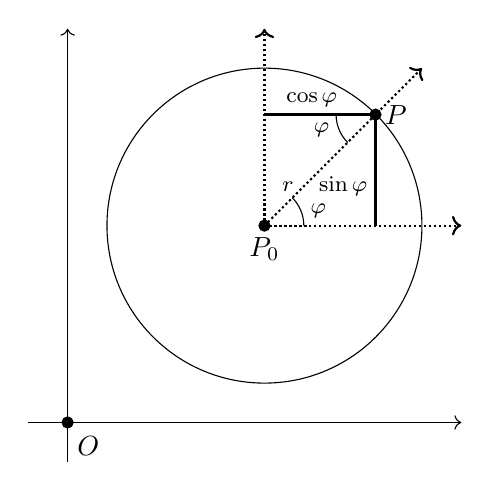
\begin{tikzpicture}
        \draw[->] (-0.5, 0) -- (5, 0);
        \draw[->] (0, -0.5) -- (0, 5);

        \draw[->, thick, densely dotted] (2.5, 2.5) -- (5, 2.5);
        \draw[->, thick, densely dotted] (2.5, 2.5) -- (4.5, 4.5);
        \draw[->, thick, densely dotted] (2.5, 2.5) -- (2.5, 5);

        \draw (3, 2.5) arc(0:45:0.5cm) node[midway, right] {\footnotesize \( \varphi \)};
        \draw (3.41, 3.91) arc(0:45:-0.5cm) node[midway, left] {\footnotesize \( \varphi \)};

        \filldraw [black] (0, 0) circle (2pt);
        \node[right] at (0, -0.3) {\( O \)};

        \draw (2.5, 2.5) circle(2);
        \filldraw [black] (2.5, 2.5) circle (2pt);
        \node at (2.5, 2.2) {\( P_0 \)};

        \filldraw [black] (3.91, 3.91) circle (2pt);
        \node[right] at (3.91, 3.91) {\( P \)};

        \draw[thick] (3.91, 3.91) -- (3.91, 2.5);
        \node at (2.8, 3) {\footnotesize \( r \)};
        \node at (3.5, 3) {\footnotesize \( \sin \varphi \)};
        \draw[thick] (3.91, 3.91) -- (2.5, 3.91);
        \node at (3.1, 4.1) {\footnotesize \( \cos \varphi \)};
      \end{tikzpicture}
      \caption{Окръжност}
    \end{figure}
  \end{minipage}
\end{definition}

\begin{definition}
  \hfill\allowbreak
  \bigskip

  \begin{minipage}{0.45\textwidth}
    \textbf{Елипса} с \textbf{фокуси} \( \Point F_0 \) и \( \Point F_1 \) и \textbf{голяма полуос} \( a > 0 \) наричаме множеството \( k \) от точки \( P \), за които е изпълнено \( \Norm{F_0 P} + \Norm{F_1 P} = 2a \).

    Разглеждаме частния случай, когато \( \Point F_0 \) и \( \Point F_1 \) имат координати \( F_0(-c, 0) \) и \( F_1(c, 0) \) спрямо \( K \) за някоя константа \( c \geq 0 \) с \( c < a \), наречена \textbf{линеен ексцентрицитет} на \( k \). За всяка елипса съществува единствена координатна система, в която уравненията на фокусите имат този прост вид. Въвеждаме следните допълнителни понятия
  \end{minipage}
  \hspace{0.5cm}
  \begin{minipage}{0.45\textwidth}
    \begin{figure}[H]\label{fig:ellipse}
      \centering
      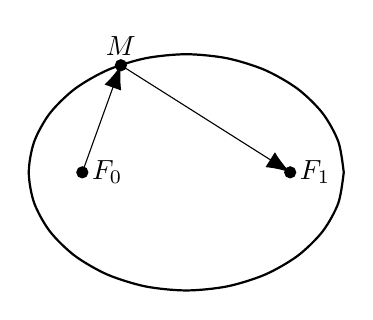
\begin{tikzpicture}
        \draw[domain=0:360, smooth, variable=\x, thick] plot ({2*cos(\x)}, {3/2*sin(\x)});

        \filldraw [black] (-1.32, 0) circle (2pt);
        \node[right] at (-1.32, 0) {\( F_0 \)};

        \filldraw [black] (1.32, 0) circle (2pt);
        \node[right] at (1.32, 0) {\( F_1 \)};

        \filldraw [black] (-0.83, 1.36) circle (2pt);
        \draw[-{Latex[length=3mm]}] (-1.32, 0) -- (-0.83, 1.36);
        \draw[-{Latex[length=3mm]}] (-0.83, 1.36) -- (1.32, 0);
        \node at (-0.83, 1.6) {\( M \)};
      \end{tikzpicture}
      \caption{Елипса}
    \end{figure}
  \end{minipage}

  \begin{itemize}
    \item Величината \( b \coloneqq \sqrt{a^2 - c^2} \) наричаме \textbf{малка полуос} на \( k \). За елипси имаме \( b = \sqrt{a^2 - c^2} \leq \sqrt{a^2} = a \).

    \item Величината \( e \coloneqq \frac c a \) наричаме \textbf{(числен) ексцентрицитет} на \( k \). За елипси имаме  \( e = \frac c a = \frac {\sqrt{a^2 - b^2}} {\sqrt{a^2}} < 1 \).

    \item \textbf{Директриси} на елипсата \( k \) наричаме правите с уравнения \( d_1: x = - \frac a e \) и \( d_2: x = \frac a e \).
  \end{itemize}

  Разписваме уравнението за \( k \) покоординатно:
  \begin{align*}
    \Norm{F_0 P} + \Norm{F_1 P} &= 2a \\
    \Norm{F_1 P} &= 2a - \Norm{F_0 P} \mid {(\cdot)}^2 \\
    \Norm{F_1 P}^2 &= 4a^2 - 4a \Norm{F_0 P} + \Norm{F_0 P}^2 \\
    4a \Norm{F_0 P} &= 4a^2 + \Norm{F_0 P}^2 - \Norm{F_1 P}^2 \mid \cdot / 4a \\
    \Norm{F_0 P} &= a + \frac {\Norm{F_0 P}^2 - \Norm{F_1 P}^2} {4a} \\
    \sqrt{{(x+c)}^2 + y^2} &= a + \frac {{(x + c)}^2 + y^2 - {(x - c)}^2 - y^2} {4a} \\
    \sqrt{{(x+c)}^2 + y^2} &= a + \frac c a x \mid {(\cdot)}^2 \\
    x^2 + 2xc + c^2 + y^2 &= a^2 + 2 xc + \frac {c^2} {a^2} x^2 \\
    \left(1 - \frac {c^2} {a^2} \right) x^2 + y^2 &= a^2 - c^2 \mid / {(a^2 - c^2)} \\
    \frac {x^2} {a^2} + \frac {y^2} {a^2 - c^2} &= 1.
  \end{align*}

  Така получаваме \textbf{метрично канонично уравнение на елипсата \( k \)} спрямо \( K \):
  \begin{equation*}
    k: \frac {x^2} {a^2} + \frac {y^2} {b^2} = 1.
  \end{equation*}

  Веднага виждаме, че елипсите са алгебрични криви от втора степен и че централното уравнение на окръжност е частен случай с \( a = b = r \iff c = 0 \).

  \textbf{Скаларни параметрични уравнения на елипса} можем да изведем аналогично на тези за окръжност. В нашия опростен случай те имат вида
  \begin{equation*}
    \begin{cases}
      x = a \cos \varphi \\
      y = b \sin \varphi
    \end{cases},
    \varphi \in [0, 2\pi).
  \end{equation*}

  \begin{theorem}[Фокално свойство на елипса]
    Всеки лъч с начало \( \Point F_0 \) след отражение в произволна точка \( M \) от елипсата минава през \( \Point F_1 \) (\cref{fig:ellipse}).
  \end{theorem}
\end{definition}

\begin{definition}
  \hfill\allowbreak
  \bigskip

  \begin{minipage}{0.45\textwidth}
    \textbf{Хипербола} с \textbf{фокуси} \( \Point F_0 \) и \( \Point F_1 \) и \textbf{реална полуос} \( a > 0 \) наричаме двусвързаното множество \( k \) от точки \( P \), за които е изпълнено \( \Abs{\Norm{F_0 P} - \Norm{F_1 P}} = 2a \).

    Разглеждаме частния случай, когато \( \Point F_0 \) и \( \Point F_1 \) имат координати \( F_0(-c, 0) \) и \( F_1(c, 0) \) спрямо \( K \) за някоя константа \( c \geq 0 \) с \( c > a \), наречена \textbf{линеен ексцентрицитет} на \( k \). За всяка хипербола съществува единствена координатна система, в която уравненията на фокусите имат този прост вид. Въвеждаме следните допълнителни понятия
  \end{minipage}
  \hspace{0.5cm}
  \begin{minipage}{0.45\textwidth}
    \begin{figure}[H]\label{fig:hyperbola}
      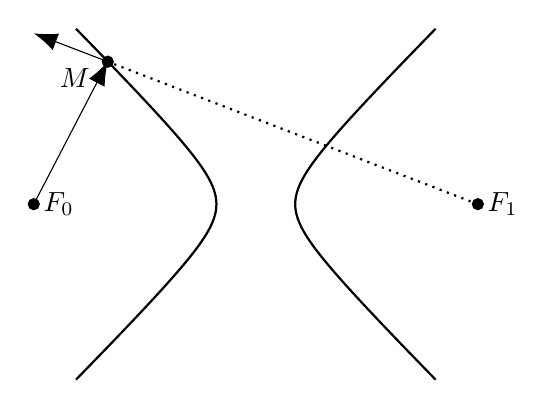
\begin{tikzpicture}
        \draw[domain=-2.2:2.2, smooth, variable=\x, thick] plot ({cosh(\x)/2}, {sinh(\x)/2});
        \draw[domain=-2.2:2.2, smooth, variable=\x, thick] plot ({-cosh(\x)/2}, {sinh(\x)/2});

        \filldraw [black] (-2.82, 0) circle (2pt);
        \node[right] at (-2.82, 0) {\( F_0 \)};

        \filldraw [black] (2.82, 0) circle (2pt);
        \node[right] at (2.82, 0) {\( F_1 \)};

        \filldraw [black] (-1.88, 1.81) circle (2pt);
        \draw[-{Latex[length=3mm]}] (-2.82, 0) -- (-1.88, 1.81);
        \draw[-{Latex[length=3mm]}] (-1.88, 1.81) -- (-2.82, 2.17);
        \draw[thick, dotted] (2.82, 0) -- (-1.88, 1.81);
        \node at (-2.3, 1.6) {\( M \)};
      \end{tikzpicture}
      \caption{Хипербола}
    \end{figure}
  \end{minipage}

  \begin{itemize}
    \item Величината \( b \coloneqq \sqrt{c^2 - a^2} \) наричаме \textbf{имагинерна полуос} на \( k \).

    \item Аналогично на елипсите, величината \( e \coloneqq \frac c a \) наричаме \textbf{(числен) ексцентрицитет} на \( k \). За хиперболи имаме  \( e = \frac c a = \frac {\sqrt{a^2 + b^2}} {\sqrt{a^2}} > 1 \).

    \item Аналогично на елипсите, \textbf{директриси} на хиперболата \( k \) наричаме правите с уравнения \( d_1: x = - \frac a e \) и \( d_2: x = \frac a e \).
  \end{itemize}

  Напълно аналогично на случая с елипса, разписвайки уравнението за \( k \) покоординатно стигаме до уравнението
  \begin{equation*}
    \frac {x^2} {a^2} + \frac {y^2} {a^2 - c^2} = 1.
  \end{equation*}

  Единствената разлика е, че тук \( b = -(a^2 - c^2) \). Така получаваме \textbf{метрично канонично уравнение} на хиперболата \( k \) спрямо \( K \):
  \begin{equation*}
    k: \frac {x^2} {a^2} - \frac {y^2} {b^2} = 1.
  \end{equation*}

  Веднага виждаме, че хиперболите са алгебрични криви от втора степен.

  \textbf{Скаларните параметрични уравнения на хипербола} са различни за левия и десния клон на хиперболата. В нашия опростен случай те имат вида
  \begin{equation*}
    \begin{cases}
      x = \pm a \cosh \varphi \\
      y = b \sinh \varphi
    \end{cases},
    \varphi \in [0, 2\pi).
  \end{equation*}

  \begin{theorem}[Фокално свойство на хипербола]
    Всеки лъч с начало \( \Point F_0 \) след отражение в произволна точка \( M \) от хиперболата лежи върху правата, минаваща през \( \Point M \) и \( \Point F_1 \) (\cref{fig:hyperbola}).
  \end{theorem}
\end{definition}

\begin{definition}
  \hfill\allowbreak
  \bigskip

  \begin{minipage}{0.45\textwidth}
    \textbf{Парабола} с \textbf{фокус} \( \Point F \) и неминаваща през \( F \) права \( d \), наречена \textbf{директриса}, наричаме множеството \( k \) от точки \( P \), за които е изпълнено \( \Norm{F P} = \Dist(d, P) \). Дефинираме \textbf{линейния и числения ексцентрицитет} на параболата \( K \) да бъдат \( c = e = 1 \).

    Разглеждаме частния случай, когато \( d \) има уравнение \( d: x = - \frac p 2 \) и \( \Point F \) има координати \( F \left(\frac p 2, 0 \right) \) спрямо \( K \) за някоя константа \( p > 0 \), наречена \textbf{параметър}. За всяка парабола съществува единствена координатна система, в която уравненията на фокуса и директрисата имат този прост вид.
  \end{minipage}
  \hspace{0.5cm}
  \begin{minipage}{0.45\textwidth}
    \begin{figure}[H]\label{fig:parabola}
      \begin{center}
        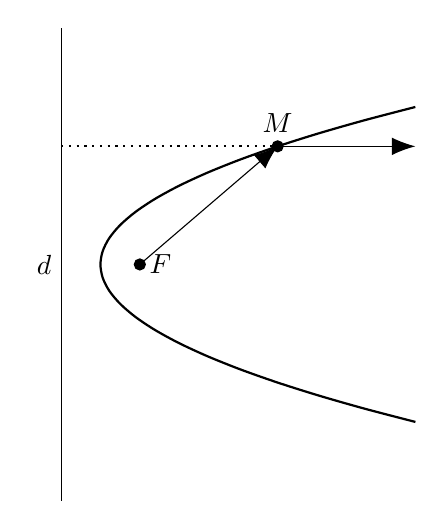
\begin{tikzpicture}
          \draw[domain=-2:2, smooth, variable=\y, thick] plot ({\y*\y}, {\y});

          \filldraw [black] (0.5, 0) circle (2pt);
          \node[right] at (0.5, 0) {\( F \)};

          \draw (-0.5, -3) -- (-0.5, 3) node[midway, left] {\( d \)};

          \filldraw [black] (2.25, 1.5) circle (2pt);
          \draw[-{Latex[length=3mm]}] (0.5, 0) -- (2.25, 1.5);
          \draw[-{Latex[length=3mm]}] (2.25, 1.5) -- (4, 1.5);
          \draw[thick, dotted] (-0.5, 1.5) -- (2.25, 1.5);
          \node at (2.25, 1.8) {\( M \)};
        \end{tikzpicture}
      \end{center}
      \caption{Парабола}
    \end{figure}
  \end{minipage}

  Нека \( \Point P \) има координати \( P(x, y) \) спрямо \( K \). Тъй като уравнението \( d: x = - \frac p 2 \) е нормално, \cref{thm:plane_distance} ни дава \( \Dist(d, P) = x + \frac p 2 \). Разписваме уравнението за \( k \) покоординатно:
  \begin{align*}
    \Norm{F P} &= \Dist(d, P) \\
    {\Norm{F P}}^2 &= {\Dist(d, P)}^2 \\
    {\left(x - \frac p 2 \right)}^2 + y^2 &= {\left(x + \frac p 2 \right)}^2 \\
    y^2 &= {\left(x + \frac p 2 \right)}^2 - {\left(x - \frac p 2 \right)}^2 \\
    y^2 &= 2px.
  \end{align*}

  Така получаваме \textbf{метрично канонично уравнение на параболата \( k \)} спрямо \( K \):
  \begin{equation*}
    k: y^2 = 2px.
  \end{equation*}

  Веднага виждаме, че параболите са алгебрични криви от втора степен.

  Ако вземем \( y \) за параметър, получаваме следните \textbf{скаларни параметрични уравнения} на параболата \( k \) спрямо \( K \):
  \begin{equation*}
    k: \begin{cases}
      x = \frac{\varphi^2} {2p} \\
      y = \varphi,
    \end{cases}
    \varphi \in \R.
  \end{equation*}

  \begin{theorem}[Фокално свойство на парабола]
    Всеки лъч с начало \( \Point F \) след отражение в произволна точка \( M \) от параболата, става перпендикулярен на директрисата \( d \) (\cref{fig:parabola}).
  \end{theorem}
\end{definition}

\section{Примерни задачи}

В конспекта не е посочен списък с възможни задачи, затова съм включил няколко по-обширни задачи от \cite{Notes}.

\subsection{Прави в равнината}

\begin{exercise}
  Точките \( A \) и \( B \) и правите \( a \) и \( b \) имат спрямо ортонормирана координатна система \( K = Oxy \) координати \( A(1, -2) \), \( B(0, -1) \) и общи уравнения
  \begin{align*}
    &a: 3x + 4y + 2 = 0, \\
    &b: 5x - 12y + 1 = 0.
  \end{align*}

  Да се намерят:
  \begin{enumerate}[label=\alph*)]
    \item Общо уравнение на правата \( l \) през \( \Point A \), успоредна на \( a \)
    \item Общо уравнение на правата \( m \) през \( \Point B \), перпендикулярна на \( b \)
    \item Общо уравнение на правата \( AB \)
    \item Координатите на \( \Point B' \), която е ортогонално симетрична на \( \Point B \) относно правата \( a \)
    \item Разстоянието от \( \Point A \) до \( a \)
    \item Общо уравнение на ъглополовящата на правите \( a \) и \( b \)
    \item Ъгълът между правите \( a \) и \( b \)
    \item Общо уравнение на правата \( t \) през \( \Point B \) и \( \Point T = a \cap b \)
    \item Да се определи положението на \( \Point A \) и \( \Point B \) спрямо правата \( a \)
  \end{enumerate}
\end{exercise}

\begin{solution}
  \begin{enumerate}[label=\alph*)]
    \item Правата \( l \) е успоредна на \( a \), следователно тя има общо уравнение от вида
    \begin{equation*}
      l: 3x + 4y + C = 0,
    \end{equation*}

    където \( C \) е подбрано спрямо условието \( l \) да минава през \( \Point A \), т.е.
    \begin{equation*}
      C = - 3 \cdot 1 - 4 \cdot (-2) = 5.
    \end{equation*}

    И така, \( l \) има общо уравнение \( l: 3x + 4y + 5 = 0 \).

    \item Правата \( m \) е перпендикулярна на \( b \), следователно нормалните вектори на \( b \) (например \( n_b(5, -12) \)) са колинеарни с \( m \). Нека \( \Point P \) има координати \( P(x, y) \) спрямо \( K \). От условието \( P \in m \iff \V{BP} \parallel n_b \) намираме общото уравнение
    \begin{align*}
      m: \det
      \begin{pmatrix}
        x & 5 \\
        y + 1 & -12
      \end{pmatrix}
      = 0
      \text{ или } m: 12x + 5y + 5 = 0.
    \end{align*}

    \item Нека \( \Point P \) има координати \( P(x, y) \) спрямо \( K \). От условието \( P \in AB \iff \V{BP} \parallel \V{BA} \) намираме общото уравнение
    \begin{align*}
      AB: \det
      \begin{pmatrix}
        x & 1 \\
        y + 1 & -1
      \end{pmatrix}
      = 0
      \text{ или } AB: x + y + 1 = 0.
    \end{align*}

    \item Нека \( B' \) има спрямо \( K \) координати \( B'(x', y') \). Първо намираме правата \( BB' \) от условието \( BB' \perp a \), което е еквивалентно на \( BB' \parallel n_a(3, 4) \). Нека \( \Point P \) има координати \( (x, y) \) спрямо \( K \). От условието \( P \in BB' \iff \V{BP} \parallel n_a \) намираме общото уравнение
    \begin{align*}
      BB': \det
      \begin{pmatrix}
        x & 3 \\
        y + 1 & 4
      \end{pmatrix}
      = 0
      \text{ или } BB': 4x - 3y - 3 = 0.
    \end{align*}

    Координатите на пресечната точка \( B_a \) на \( a \) и \( BB' \) (ортогоналната проекция на \( B \) върху \( a \)) намираме от системата
    \begin{equation*}
      \begin{cases}
        3x + 4y + 2 = 0 \mid (\times 3) \\
        4x - 3y - 3 = 0 \mid (\times 4)
      \end{cases}
      \sim
      \begin{cases}
        9x + 12y + 6 = 0 \\
        16x - 12y - 12 = 0
      \end{cases}
      \sim
      \begin{cases}
        25x = 6 \\
        12y = 16x - 12
      \end{cases},
    \end{equation*}

    откъдето получаваме \( B_a(6/25, -17/25) \).

    Остава да намерим координатите на \( B' \). Имаме \( \V{BB_a} = \V{B_a B'} \), откъдето
    \begin{equation*}
      \begin{cases}
        6/25 = x' - 6/25 \\
        -17/25 + 1 = y' + 17/25
      \end{cases}
      \sim
      \begin{cases}
        x' = 12/25 \\
        y' = -34/25 + 1 = -9/25
      \end{cases}.
    \end{equation*}

    Получихме \( B'(12/25, -9/25) \).

    \item Разстоянието \( \Dist(A, a) \) намираме използвайки \cref{thm:plane_distance}:
    \begin{equation*}
      \Dist(A, a) = \Abs{\ODist(A, a)} = \frac {\Abs{F_a(A)}} {\Norm {n_a}},
    \end{equation*}

    където \( F_a(x, y) = 3x + 4y + 2 \) е лявата част на зададеното общо уравнение на \( a \), а \( n_a(3, 4) \) е съответният нормален вектор. Директно пресмятаме разстоянието и получаваме
    \begin{equation*}
      \Dist(A, a) = \frac {\Abs{3 \cdot 1 + 4 \cdot (-2) + 2}} 5 = \frac 3 5.
    \end{equation*}

    \item Ъглополовящите \( u_{1,2} \) на правите \( a \) и \( b \) се състоят от всички точки \( P(x, y) \), за които \( \Dist(P, a) = \Dist(P, b) \). Последното условие е еквивалентно на условието \( \ODist(P, a) \pm \ODist(P, b) = 0 \), откъдето намираме уравненията на ъглополовящите:
    \begin{align*}
      u_{1,2}&: \frac {3x + 4y + 2} 5 \pm \frac {5x - 12y + 1} {13} = 0, \\
      u_{1,2}&: (39x + 52y + 26) \pm (25x - 60y + 5) = 0, \\
      u_1&: 64x - 8y + 31 = 0, \\
      u_2&: 14x + 112y + 21 = 0.
    \end{align*}

    \item Ъгълът между \( a \) и \( b \) намираме чрез нормалните им вектори \( n_a(3, 5) \) и \( n_b(5, -12) \):
    \begin{equation*}
      \angle(a, b) = \arccos \frac {\Abs{\Prod{n_a} {n_b}}} {\Norm{n_a} \Norm{n_b}} = \arccos \Abs {- \frac {33} {65}} = \arccos \frac {33} {65}
    \end{equation*}

    \item Координатите на пресечната точка \( T \) на \( a \) и \( b \) намираме от системата
    \begin{equation*}
      \begin{cases}
        3x + 4y + 2 = 0 \mid (\times 3) \\
        5x - 12y + 1 = 0
      \end{cases}
      \sim
      \begin{cases}
        9x + 12y + 6 = 0 \\
        5x - 12y + 1 = 0
      \end{cases}
      \sim
      \begin{cases}
        14x = -7 \\
        12y = 5x + 1
      \end{cases}
    \end{equation*}

    откъдето получаваме \( T(-1/2, -1/8) \).

    Нека \( \Point P \) има координати \( (x, y) \) спрямо \( K \). От условието \( P \in t \iff \V{TP} \parallel \V{TB} \) намираме общото уравнение
    \begin{align*}
      t: \det
      \begin{pmatrix}
        x + 1/2 & 1/2 \\
        y + 1/8 & -7/8
      \end{pmatrix}
      =
      \frac 1 {16}
      \begin{pmatrix}
        2x + 1 & 1 \\
        8y + 1 & -7
      \end{pmatrix}
      = -14x - 8y - 8 = 0
    \end{align*}
    или \( t: 7x + 4y + 4 = 0 \).

    \item Означаваме \( F_a(x, y) = 3x + 4y + 2 \). Имаме, че \( F_a(A) = F_a(1, -2) = -3 < 0 \) и \( F_a(B) = F_a(0, -1) = -2 < 0 \). Двете точки не лежат върху правата \( a \) и освен това \( F_a(A) \) и \( F_a(B) \) имат еднакви знаци, следователно \( \Point A \) и \( \Point B \) лежат в една и съща отворена полуравнина относно \( a \).
  \end{enumerate}
\end{solution}

\bigskip
\begin{minipage}{0.45\textwidth}
    \begin{exercise}
    В равнината е зададена ортонормирана координатна система \( K = Oxy \). Дадени са правите
    \begin{align*}
      &a: x + y = 0 \\
      &b: x - 3y - 2 = 0
    \end{align*}

    Светлинен лъч \( l \Ray \) минава през точка \( M(2, 2) \) и се отразява от правата \( a \). Отразеният лъч \( l' \Ray \) е колинеарен с правата \( b \).

    Да се намерят уравнения спрямо \( K \) на правите \( l \) и \( l' \), съдържащи съответно падащия лъч \( l \Ray \) и отразения лъч \( l' \Ray \).
  \end{exercise}
\end{minipage}
\hspace{0.5cm}
\begin{minipage}{0.45\textwidth}
  \begin{figure}[H]\label{fig:plane_light_ray}
    \centering
    \begin{tikzpicture}[rotate=45]
      \filldraw [black] (2, 2) circle (2pt);
      \node[right] at (2, 2) {\( M(2, 2) \)};

      \filldraw [black] (0, 0) circle (2pt);
      \node at (1/3, 1/3) {\( M_a \)};

      \filldraw [black] (-2, -2) circle (2pt);
      \node[right] at (-2, -2) {\( M' \)};

      \filldraw [black] (1, -1) circle (2pt);
      \node at (1.5, -1.1) {\( N \)};

      \node[right] at (5/3, 1) {\( l \)};
      \draw[-{Latex[length=3mm]}] (7/3, 3) -- (1, -1);
      \draw[thick, dotted] (1, -1) -- (-1/3, -5);

      \node[right] at (3, -1/3) {\( l' \)};
      \draw[-{Latex[length=3mm]}] (1, -1) -- (5, 1/3);
      \draw[thick, dotted] (-3, -7/3) -- (1, -1);

      \node[right] at (-7/10, 1) {\( a \)};
      \draw[-] (-6/5, 6/5) -- (3, -3);

      \node[right] at (3, 1/3) {\( b \)};
      \draw[dotted] (-3, -5/3) -- (13/3, 7/9);
    \end{tikzpicture}
    \caption{Отразен светлинен лъч}
  \end{figure}
\end{minipage}
\bigskip

\begin{solution}
  \mbox{}
  \begin{enumerate}
    \item Намираме координатите на ортогоналната проекция \( M_a \) на точката \( M \) върху \( a \), използвайки нормален за \( a \) вектор \( n_a(1, 1) \).

    От условието \( n_a \parallel \V{M M_a} \) намираме ограничението
    \begin{align*}
      M_a(x, y): \det
      \begin{pmatrix}
        1 & x - 2 \\
        1 & y - 2
      \end{pmatrix}
      = y - x
      = 0,
    \end{align*}

    а от ограничението \( M_a \in a \) получаваме, че \( \Point M_a \) има координати \( (0, 0) \) спрямо \( K \).

    \item Намираме координатите на ортогонално симетричната точка \( M'(x', y') \) на \( M \) относно \( a \). Имаме \( \V{MM_a} = \V{M_a M'} \), откъдето
    \begin{equation*}
      \begin{cases}
        2 - 0 = 0 - x' \\
        2 - 0 = 0 - y'
      \end{cases}
      \implies
      x' = y' = -2,
    \end{equation*}
    т.е. \( M'(-2, -2) \).

    \item Намираме уравнението на правата \( l' \). Тъй като \( l' \parallel b \), правата \( l' \) има общо уравнение
    \begin{equation*}
      l': x - 3y + C = 0,
    \end{equation*}

    където \( C \) е подбрано спрямо условието \( l' \) да минава през \( \Point M' \), т.е.
    \begin{equation*}
      C = - 1 \cdot (-2) + 3 \cdot (-2) = -4.
    \end{equation*}

    И така, \( l' \) има общо уравнение \( l': x - 3y - 4 = 0 \).

    \item Намираме координатите на пресечната точка \( N \) на \( a \) и \( l' \) (а също и \( l' \)):
    \begin{equation*}
      N(x, y): \begin{cases}
        x + y = 0 \\
        x - 3y - 4 = 0
      \end{cases}
      \sim
      \begin{cases}
        x = -y \\
        -4y = 4
      \end{cases}
      \sim
      \begin{cases}
        x = 1 \\
        y = -1
      \end{cases},
    \end{equation*}

    т.е. \( N(1, -1) \).

    \item Намираме общо уравнение на \( l \). Използваме това, че \( l \) минава през \( \Point M \) и \( \Point N \), т.е. \( \Point P(x, y) \in l \iff \V{MP} \parallel \V{MN} \):
    \begin{align*}
      l: \det
      \begin{pmatrix}
        x - 2 & 1 - 2\\
        y - 2 & -1 - 2
      \end{pmatrix}
      =
      -3x + y + 4
      =
      0.
    \end{align*}
  \end{enumerate}
\end{solution}

\subsection{Равнини в пространството}

\begin{exercise}
  В пространството е зададена ортонормирана координатна система \( K = Oxyz \). Спрямо нея точките \( A \), \( B \), \( C \) и \( D \) имат координати
  \begin{align*}
    &A(3, 1, 4) &C(1, 2, -1) \\
    &B(2, 1, 3) &D(0, -3, 2),
  \end{align*}

  а равнината \( \beta \) има общо уравнение
  \begin{equation*}
    \beta: x + y - z + 1 = 0.
  \end{equation*}

  Да се намерят:
  \begin{enumerate}[label=\alph*)]
    \item Общо уравнение на равнината \( \alpha \), минаваща през точките \( A \), \( B \) и \( C \)
    \item Параметрични уравнения на права \( h \), минаваща през \( \Point D \) и ортогонална на равнината \( \alpha \)
    \item Координатите на ортогонално симетричната на \( \Point D \) спрямо \( \alpha \) точка \( \Point D' \)
    \item Общо уравнение на равнината \( \gamma \), минаваща през \( \Point D \) и успоредна на \( \beta \)
    \item Координатите на някой вектор \( v \), компланарен с \( \alpha \) и \( \beta \)
    \item Параметрични уравнения на пресечницата \( m \) на \( \alpha \) и \( \beta \)
    \item Параметрични уравнения на права \( l \), така че светлинния лъч \( l\Ray \) през \( \Point D \) след отразяването си от \( \alpha \) (озн. отразения лъч с \( l'\Ray \)) пресича \( \beta \) под прав ъгъл
    \item Общо уравнение на равнината \( \pi_1 \), минаваща през \( A \) и ортогонална на правата \( m \)
    \item Общо уравнение на равнината \( \pi_2 \), съдържаща правата \( l' \) и успоредна на правата \( m \)
    \item Общо уравнение на равнината \( \pi_3 \), съдържаща правата \( l' \) и ортогонална на равнината \( \alpha \)
  \end{enumerate}
\end{exercise}

\begin{solution}
  \begin{enumerate}[label=\alph*)]
    \item Нека \( \Point P(x, y, z) \in \alpha \). Тогава \( \V{AP} \parallel \V{AB}(-1, 0, -1) \parallel \V{AC}(-2, 1, -5) \), което условие ни позволява да намерим общо уравнение на \( \alpha \):
    \begin{align*}
      \alpha: &\det
      \begin{pmatrix}
        x - 3 & -1 & -2 \\
        y - 1 & 0 & 1 \\
        z - 4 & -1 & -5
      \end{pmatrix}
      = \\ &=
      -1(z-4) + (-2)(y-1)(-1) - (x-3)(-1) - (-1)(y-1)(-5)
      = \\ &=
      -z + 4 + 2y - 2 + x - 3 - 5y + 5
      = \\ &=
      \boxed{x - 3y - z + 4 = 0}.
    \end{align*}

    \item Правата \( h \) е успоредна на нормалния за \( \alpha \) вектор на \( n_\alpha(1, -3, -1) \), следователно тя има векторно параметрично уравнение
    \begin{equation*}
      h: \V{OD} + \lambda n_\alpha, \lambda \in \R
    \end{equation*}
    и, съответно, скаларно параметрично уравнение
    \begin{equation*}
      h: \begin{cases}
        x = \lambda \\
        y = -3 - 3\lambda \\
        z = 2 - \lambda
      \end{cases},
      \lambda \in \R.
    \end{equation*}

    \item За да намерим ортогонално симетричната на \( \Point D \) спрямо \( \alpha \) точка \( \Point D'(x', y', z') \), първо ще намерим пресечната точка \( \Point D_\alpha \) на правата \( h \) и равнината \( \alpha \).

    Намираме стойността на параметъра \( \lambda \) за уравнението на \( h \), за която \( h \) се пресича \( \alpha \):
    \begin{align*}
      \lambda - 3(-3 - 3\lambda) - (2 - \lambda) + 4 &= 0 \\
      \lambda + 9 + 9\lambda - 2 + \lambda + 4 &= 0 \\
      11 \lambda &= -11 \\
      \lambda &= -1,
    \end{align*}

    откъдето намираме координатите \( (-1, 0, 3) \) на \( \Point D_\alpha \).

    След това, развиваме очевидното равенство \( \V{D_\alpha D'} = \V{DD_\alpha} \) покоординатно:
    \begin{equation*}
      \begin{cases}
        x' + 1 = -1 \\
        y' - 0 = 3 \\
        z' - 3 = 1
      \end{cases}
      \sim
      \begin{cases}
        x' = -2 \\
        y' = 3 \\
        z' = 4,
      \end{cases}
    \end{equation*}
    т.е. \( D'(-2, 3, 4) \).

    \item Тъй като равнината \( \gamma \) е успоредна на \( \beta \), тя има общо уравнение
    \begin{equation*}
      \gamma: x + y - z + C = 0,
    \end{equation*}

    където \( C \) е подбрано спрямо условието \( \gamma \) да минава през \( \Point D \), т.е.
    \begin{equation*}
      C = -(0 + (- 3) - 2) = 5.
    \end{equation*}

    И така, \( \gamma: x + y - z + 5 = 0 \).

    \item Търсим едновременни решения на известните общи уравнения на равнините \( \alpha \) и \( \beta \):
    \begin{equation*}
      \begin{cases}
        \alpha: x - 3y - z + 4 = 0 \\
        \beta: x + y - z + 1 = 0
      \end{cases}
      \sim
      \begin{cases}
        y = 3 / 4 \\
        z = x + 7 / 4.
      \end{cases}
    \end{equation*}

    Очевидно точките \( V_0\left(0, \frac 3 4, \frac 7 4 \right) \) и \( V_1\left( 1, \frac 3 4, 1 + \frac 7 4 \right) \) удовлетворяват горната система, следователно векторът \( v = \V{V_0 V_1} \) с координати \( (1, 0, 1) \) е колинеарен и с двете равнини.

    \item Пресечницата \( m \) на \( \alpha \) и \( \beta \) има векторно параметрично уравнение
    \begin{equation*}
      m: \V{OV_0} + \mu v, \mu \in \R
    \end{equation*}
    и, съответно, скаларно параметрично уравнение
    \begin{equation*}
      m: \begin{cases}
        x = \mu \\
        y = 3/4 \\
        z = 7/4 + \mu
      \end{cases},
      \mu \in \R.
    \end{equation*}

    \item Тъй като вече разполагаме с координатите на ортогонално симетричната на \( D \) относно \( \alpha \) точка \( D' \) и нормалният за \( \alpha \) вектор \( n_\beta(1, 1, -1) \), можем да намерим векторно параметрично уравнения на правата \( l' \):
    \begin{equation*}
      l': \V{OD'} + \nu n_\beta, \nu \in \R
    \end{equation*}
    и, съответно, скаларното параметрично уравнение
    \begin{equation*}
      l': \begin{cases}
        x = -2 + \nu \\
        y = 3 + \nu \\
        z = 4 - \nu
      \end{cases},
      \nu \in \R.
    \end{equation*}

    Сега намираме стойността на параметъра \( \nu \), за която \( l' \) пресича равнината \( \alpha \):
    \begin{align*}
      (-2 + \nu) - 3(3 + \nu) - (4 - \nu) + 4 &= 0 \\
      -2 + \nu - 9 - \nu - 4 + \nu + 4 &= 0 \\
      \nu &= 11
    \end{align*}
    т.е. пресечната точка \( N \) на \( l' \) и \( \alpha \) има координати \( N(9, 14, -7) \).

    Сега намираме векторно параметрично уравнения на правата \( l \), минаваща през \( \Point D \) и \( \Point N \):
    \begin{equation*}
      l: \V{OD} + \xi \V{DN}, \xi \in \R
    \end{equation*}
    и, съответно, скаларното параметрично уравнение
    \begin{equation*}
      l: \begin{cases}
        x = 9\xi \\
        y = -3 + 17\xi \\
        z = 2 - 9\xi
      \end{cases},
      \xi \in \R.
    \end{equation*}

    \item Първо намираме два нормални за правата \( m \) вектора. Нека \( u(x, y, z) \) е произволен вектор. Тъй като \( v \) е направляващ за \( m \), \( u \) е нормален за \( m \) само ако
    \begin{equation*}
      \Prod u v = x + z = 0.
    \end{equation*}

    От горното условие виждаме, че два нормални за \( m \) вектора са \( u_1(0, 1, 0) \) и \( u_2(-1, 0, 1) \).

    Нека \( \Point P \) има спрямо \( K \) координати \( (x, y, z) \). Тогава \( \Point P \in \pi_1 \) точно тогава, когато векторът \( \V{AP} \) е колинеарен с \( u_1 \) и \( u_2 \), т.е.
    \begin{align*}
      \pi_1: \det
      \begin{pmatrix}
        x - 3 & 0 & -1 \\
        y - 1 & 1 & 0 \\
        z - 4 & 0 & 1
      \end{pmatrix}
      = (x - 3) - (-1)(z - 4) = \boxed{x + z - 7 = 0}.
    \end{align*}

    \item Имаме, че \( \Point D'(-2, 3, 4) \in l' \) и векторът \( n_\beta(1, 1, -1)' \) е направляващ за \( l' \), а \( v(1, 0, 1) \) е направляващ за \( m \). Нека \( \Point P \) има спрямо \( K \) координати \( (x, y, z) \). Тогава \( \Point P \in \pi_2 \) точно тогава, когато са колинеарни векторите \( \V{D'P} \), \( n_\beta \) и \( v \), т.е.
    \begin{align*}
      &\pi_2: \det
      \begin{pmatrix}
        x + 2 & 1  & 1 \\
        y - 3 & 1  & 0 \\
        z - 4 & -1 & 1
      \end{pmatrix}
      = \\ &=
      (x + 2) + (y - 3)(-1) - (z - 4) - (y - 3)
      = \\ &=
      \boxed{x - 2y - z + 12 = 0}.
    \end{align*}

    \item Аналогично на \( \pi_2 \), имаме, че \( \Point P \in \pi_3 \) точно тогава, когато са колинеарни векторите \( \V{D'P} \), \( n_\beta \) и \( n_\alpha(1, -3, -1) \)
    \small{
    \begin{align*}
      &\pi_3: \det
      \begin{pmatrix}
        x + 2 & 1  & 1 \\
        y - 3 & 1  & -3 \\
        z - 4 & -1 & -1
      \end{pmatrix}
      = \\ &=
      (x + 2)(-1) + (-3)(z - 4) + (y - 3)(-1) - (z - 4) - (y - 3)(-1) - (x + 2)(-3)(-1)
      = \\ &=
      (-4)(x + 2) + (-4)(z - 4) = 0
      \\&\text{ или }
      \boxed{\pi_3: x + z - 2 = 0}.
    \end{align*}
    }
  \end{enumerate}
\end{solution}

\subsection{Прави в пространството}

\begin{exercise}
  В пространството е зададена ортонормирана координатна система \( K = Oxyz \). Спрямо нея кръстосаните прави \( g \) и \( h \) имат скаларни параметрични уравнения
  \begin{align*}
    g: \begin{cases}
      x = 1 + 2\lambda \\
      y = 4 + 4\lambda \\
      z = 4 + \lambda
    \end{cases},
    \lambda \in \R
    &&
    h: \begin{cases}
      x = -1 \\
      y = -1 - 5\mu \\
      z = 1 + 3\mu
    \end{cases},
    \mu \in \R.
  \end{align*}

  Да се намери (скаларно) параметрично уравнение на трансверзалата \( t \) на \( g \) и \( h \), за която:
  \begin{enumerate}[label=\alph*)]
    \item Точката \( A(1, 1, 1) \) лежи върху \( t \)
    \item \( t \) лежи в равнината \( \alpha: 2x + y - 3z + 6 = 0 \)
    \item \( t \) е успоредна на правата
    \begin{equation*}
      a: \begin{cases}
        x + 5y + 4z - 3 = 0 \\
        2x - 5y - 4z + 1 = 0
      \end{cases}
    \end{equation*}
  \end{enumerate}
\end{exercise}

\begin{solution}
  Тъй като правата \( t \) е трансверзала на \( g \) и \( h \), тя има по една обща точка с двете прави. Да означим тези точки с \( G \) и \( H \), т.е.
  \begin{align*}
    t \cap g = \{ G(x_g, y_g, z_g) \}
    &&
    t \cap h = \{ H(x_h, y_h, z_h) \}.
  \end{align*}

  Тъй като \( G \in g \) и \( H \in h \), то техните координати удовлетворяват уравненията на \( g \) и \( h \) за някои стойности на параметрите \( \lambda \) и \( \mu \), т.е.
  \begin{align*}
    &G(1 + 2\lambda_G, 4 + 4\lambda_G, 4 + 4\lambda_G) \\
    &H(-1, -1 -5\mu_H, 1 + 3\mu_H).
  \end{align*}

  Тогава векторът \( \V{HG} \) има координати \( \V{HG}(2 + 2\lambda_G, 5 + 4\lambda_G + 5\mu_H, 3 + \lambda_G - 3\mu_H) \).

  \begin{enumerate}[label=\alph*)]
    \item За да принадлежи точката \( A \) на трансверзалата \( t \), искаме векторите \( \V{AG}(2\lambda_G, 3 + 4\lambda_G, 3 + \lambda_G) \) и \( \V{AH}(-2, -2 - 5\mu_H, 3\mu_H) \) да бъдат колинеарни, т.е. \( \exists k \in \R \setminus \{ 0 \}: \V{AG} = k\V{AH} \). Разписваме това уравнение покоординатно:
    \begin{align*}
      &\begin{cases}
        2\lambda_G = -2k \mid (\times 1 / 2) \\
        3 + 4\lambda_G = -2k - 5k\mu_H \mid \text{ изваждаме третото уравнение} \\
        3 + \lambda_G = 3k\mu_H
      \end{cases}
      \sim \\ \sim
      &\begin{cases}
        \lambda_G = -k \\
        3\lambda_G = -2k - 8k\mu_H \\
        3 + \lambda_G = 3k\mu_H
      \end{cases}.
    \end{align*}

    От второто уравнение получаваме
    \begin{equation*}
      -k = -8k\mu_H \implies \mu_H = 1 / 8 \implies H(-1, -13/8, 11/8).
    \end{equation*}

    Правата \( t \) има векторно параметрично уравнение
    \begin{equation*}
      t: \V{OA} + 8 \nu \V{AH}, \nu \in \R
    \end{equation*}
    и, съответно, скаларно параметрично уравнение
    \begin{equation*}
      t: \begin{cases}
        x = 1 - 16\nu \\
        y = 1 - 21 \nu \\
        z = 1 + 3 \nu
      \end{cases},
      \nu \in \R.
    \end{equation*}

    \item Намираме \( \lambda_G \) и \( \mu_H \) като директно заместваме координатите на \( G \) и \( H \) в уравнението на \( \alpha \):
    \begin{align*}
      2(1 + 2\lambda_G) + (4 + 4\lambda_G) - 3(4 + \lambda_G) + 6 &= 0 \\
      2 + 4\lambda_G + 4 + 4\lambda_G - 12 + 3\lambda_G + 6 &= 0 \\
      5\lambda_G &= 0,
    \end{align*}
    следователно \( \lambda_G = 0 \) и \( \Point G \) има координати \( G(1, 4, 4) \).
    \begin{align*}
      2(-1) + (-1 - 5\mu_H) - 3(1 + 3\mu_H) + 6 &= 0 \\
      -2 - 1 - 5\mu_H - 3 - 9\mu_H + 6 &= 0 \\
      -14\mu_H &= 0,
    \end{align*}
    следователно \( \mu_H = 0 \) и \( \Point H \) има координати \( H(-1, -1, 1) \).

    Правата \( t \) има векторно параметрично уравнение
    \begin{equation*}
      t: \V{OG} + \nu \V{GH}, \nu \in \R
    \end{equation*}
    и, съответно, скаларно параметрично уравнение
    \begin{equation*}
      t: \begin{cases}
        x = 1 - 2\nu \\
        y = 4 - 5\nu \\
        z = 4 - 3\nu
      \end{cases},
      \nu \in \R.
    \end{equation*}

    \item Първо намираме скаларно параметрично уравнение на правата \( a \). Събирайки двете уравнения, получаваме
    \begin{align*}
      &\begin{cases}
        x + 5y + 4z - 3 = 0 \\
        2x - 5y - 4z + 1 = 0 \mid \text{ прибавяме първото уравнение}
      \end{cases}
      \sim \\ \sim
      &\begin{cases}
        4z = 3 - x - 5y = 7 / 3 - 5y \\
        x = 2 / 3
      \end{cases}.
    \end{align*}

    Параметризираме горната система чрез \( \xi \in \R \), полагайки \( y = 4\xi \), и получаваме
    \begin{equation*}
      a: \begin{cases}
        x = 2 / 3 \\
        y = 4\xi \\
        z = 7/{12} - 5\xi
      \end{cases},
      \xi \in \R.
    \end{equation*}

    Означаваме направляващия вектор от горното уравнение чрез \( v_a(0, 4, -5) \). За да бъдат колинеарни правите \( t \) и \( a \) е достатъчно двойка техни направляващи вектори да бъдат колинеарни, т.е. \( \V{GH} \parallel v_a \iff \exists k \in \R \setminus \{ 0 \} : \V{GH} = k v_a \). Разписвайки това уравнение само за първата координата, получаваме
    \begin{equation*}
      2 + 2\lambda_G = 0 \cdot k \implies \lambda_G = -1 \implies G(-1, 0, 3).
    \end{equation*}

    Разполагайки с точка \( G \in t \) и направляващ вектор \( v_a \parallel t \), за трансверзалата \( t \) получаваме векторно параметрично уравнение
    \begin{equation*}
      t: \V{OG} + \nu v_a, \nu \in \R
    \end{equation*}
    и, съответно, скаларно параметрично уравнение
    \begin{equation*}
      t: \begin{cases}
        x = -1 \\
        y = 4\nu \\
        z = 3 - 5\nu
      \end{cases},
      \nu \in \R.
    \end{equation*}
  \end{enumerate}
\end{solution}

\subsection{Канонизиране на криви от втора степен}

\begin{exercise}
  Спрямо ортонормирана координатна система \( K = Oxy \) е зададена кривата
  \begin{equation*}
    c: 4x^2 - 4xy + y^2 + 2x - 16y - 8 = 0.
  \end{equation*}

  Да се намери метрично канонично уравнение на \( c \) и да намерят координатите на фокусите на \( c \) спрямо \( K \).
\end{exercise}

\begin{solution}
  \begin{enumerate}
    \item Търсим ортонормирана координатна система \( K' \), в която уравнението на кривата \( c \) да няма смесен квадратен член \( xy \). Означаваме матрицата на квадратичната форма \( 4x^2 - 4xy + y^2 \) с
    \begin{align*}
      A = \begin{pmatrix}
        4 & -2 \\
        -2 & 1
      \end{pmatrix}.
    \end{align*}

    Търсим собствените вектори на \( A \):
    \begin{align*}
      \begin{pmatrix}
        4 & -2 \\
        -2 & 1
      \end{pmatrix}
      \begin{pmatrix}
        x \\ y
      \end{pmatrix}
      =
      \lambda
      \begin{pmatrix}
        x \\ y
      \end{pmatrix},
    \end{align*}
    което уравнение е еквивалентно на системата
    \begin{equation}
      \label{ex:canonization/eigen}
      \begin{cases}
        4x - 2y = \lambda x \\
        -2x + y = \lambda y
      \end{cases}
      \sim
      \begin{cases}
        -2y = (\lambda - 4) x \\
        (1 - \lambda) y = 2x
      \end{cases}
      \sim
      \begin{cases}
        y = \frac {4 - \lambda} 2 x \\
        y = \frac 2 {1 - \lambda} x.
      \end{cases}
    \end{equation}

    За да получим нормирани собствени вектори, искаме
    \begin{align*}
      x^2 + y^2 &= 1 \\
      \left(1 +  \frac 4 {{(1 - \lambda)}^2} \right) x^2 &= 1 \\
      \frac {\lambda^2 - 2\lambda + 5} {{(1 - \lambda)}^2} x^2 &= 1.
    \end{align*}
    За определеност взимаме само една двойка корени
    \begin{equation}
      \label{ex:canonization/normed_eigen}
      x = \frac {1 - \lambda} {\sqrt{\lambda^2 - 2\lambda + 5}}
      \text{ и }
      y = \frac 2 {\sqrt{\lambda^2 - 2\lambda + 5}}
    \end{equation}

    Изваждайки двете уравнения в \eqref{ex:canonization/eigen}, стигаме до характеристичния полином на \( A \):
    \begin{equation*}
      \frac {4 - \lambda} 2 - \frac 2 {1 - \lambda} = 0 \iff 4 - \lambda - 4\lambda + \lambda^2 - 4 = \lambda^2 - 5\lambda = 0,
    \end{equation*}
    чиито корени са \( \lambda_1 = 0 \) и \( \lambda_1 = 5 \), а замествайки в \eqref{ex:canonization/normed_eigen}, директно получаваме собствените вектори
    \begin{align*}
      v_1 \left(\frac 1 {\sqrt 5}, \frac 2 {\sqrt 5} \right)
      &&
      v_2 \left(\frac {-2} {\sqrt 5}, \frac 1 {\sqrt 5} \right).
    \end{align*}

    Желаната ротация има вида
    \begin{equation*}
      R: \begin{cases}
        x = \frac 1 {\sqrt 5} (x' - 2y') \\
        y = \frac 1 {\sqrt 5} (2x' + y').
      \end{cases}
    \end{equation*}

    Спрямо новата координатна система \( K' \) кривата \( c \) има вида
    \begin{equation*}
      c: 5y'^2 + \frac 2 {\sqrt 5} (x' - 2y') - \frac {16} {\sqrt 5} (2x' + y') - 8 = 5y'^2 - \frac {30} {\sqrt 5} x' - \frac {20} {\sqrt 5} y' - 8 = 0,
    \end{equation*}
    което можем да опростим до
    \begin{equation*}
      c: 5 \sqrt 5 y'^2 - 30 x' - 20 y' - 8 \sqrt 5 = 0,
    \end{equation*}

    \item Имаме уравнения на парабола, но то не е канонично. Търсим афинна координатна система \( K'' \), в която параболата да е центрирана, т.е. търсим транслация
    \begin{equation*}
      T: \begin{cases}
        x' = x'' + a \\
        y' = y'' + b,
      \end{cases}
    \end{equation*}
    така че в новата координатна система уравнението да има вида \( c: y'' = 2px'' \) за някое число \( p \).

    Правим транслацията и след това намираме подходящи стойности за параметрите \( a \) и \( b \):
    \begin{align*}
      5 \sqrt 5 y'^2 - 30 x' - 20 y' - 8 \sqrt 5 &= 0 \\
      5 \sqrt 5 y''^2 + 10 \sqrt 5 y'' b + 5 \sqrt 5 b^2 - 30 x'' - 30a - 20 y'' - 20b - 8 \sqrt 5 &= 0 \\
      5 \sqrt 5 y''^2 + (10 \sqrt 5 b - 20) y'' = 30 x'' + (- 5 \sqrt 5 b^2 + 30a + 20b + 8 \sqrt 5).
    \end{align*}

    Приравняваме на нула коефициента пред \( y'' \) и свободния коефициент:
    \begin{equation*}
      10 \sqrt 5 b - 20 = 0 \implies b = \frac 2 {\sqrt 5}
    \end{equation*}
    \begin{equation*}
      a
      =
      \frac {5 \sqrt 5 b^2 - 20 b - 8 \sqrt 5} {30}
      =
      \frac {4 \sqrt 5 - \frac {40} {\sqrt 5} - 8 \sqrt 5} {30}
      =
      \frac {20 - 40 - 40} {30 \sqrt 5}
      =
      \frac {-60} {30 \sqrt 5}
      =
      \frac {-2} {\sqrt 5}.
    \end{equation*}

    Тогава за композираната смяна на координатната система от \( K'' \) към \( K \) получаваме
    \begin{equation*}
      R \circ T: \begin{cases}
        x = \frac 1 {\sqrt 5} \left( x'' + a - 2y'' - 2b \right) \\
        y = \frac 1 {\sqrt 5} \left( 2x'' + 2a + y'' + b \right)
      \end{cases}
      \sim
      \begin{cases}
        x = \frac 1 {\sqrt 5} \left( x'' - 2y'' - \frac 6 {\sqrt 5} \right) \\
        y = \frac 1 {\sqrt 5} \left( 2x'' + y'' - \frac 2 {\sqrt 5} \right)
      \end{cases}
    \end{equation*}

    и спрямо \( K'' \) параболата има уравнение
    \begin{equation*}
      c: 5 \sqrt 5 y''^2 = 30x''
      \iff
      c: y''^2 = 2 \cdot \frac 3 {\sqrt 5}x''
    \end{equation*}

    \item Фокусът на параболата \( c \) има спрямо \( K'' \) координати \( F \left(\frac 3 {2 \sqrt 5}, 0 \right) \). Спрямо \( K \) фокусът има координати
    \begin{equation*}
      R \circ T: \begin{cases}
        x = \frac 1 {\sqrt 5} \left( \frac 3 {2 \sqrt 5} - \frac 6 {\sqrt 5} \right) = - \frac 9 {10} \\
        y = \frac 1 {\sqrt 5} \left( \frac 3 {\sqrt 5} - \frac 2 {\sqrt 5} \right) = \frac 1 5
      \end{cases},
    \end{equation*}

    т.е. \( F \left(-\frac 9 {10}, \frac 1 5 \right) \).
  \end{enumerate}
\end{solution}

\printbibliography

\end{document}
